

%%%%%%%%%%%%%%%%%%%%%%                                          About GAN                    
\begin{frame}[fragile]{Generative Adversarial Network}
 GANs are generative models: they create new data instances that resemble your training data. \\
 eg: images that look like photographs of human faces, even though the faces don't belong to any real person.
     \begin{figure}[ht]
      \hspace*{-1cm}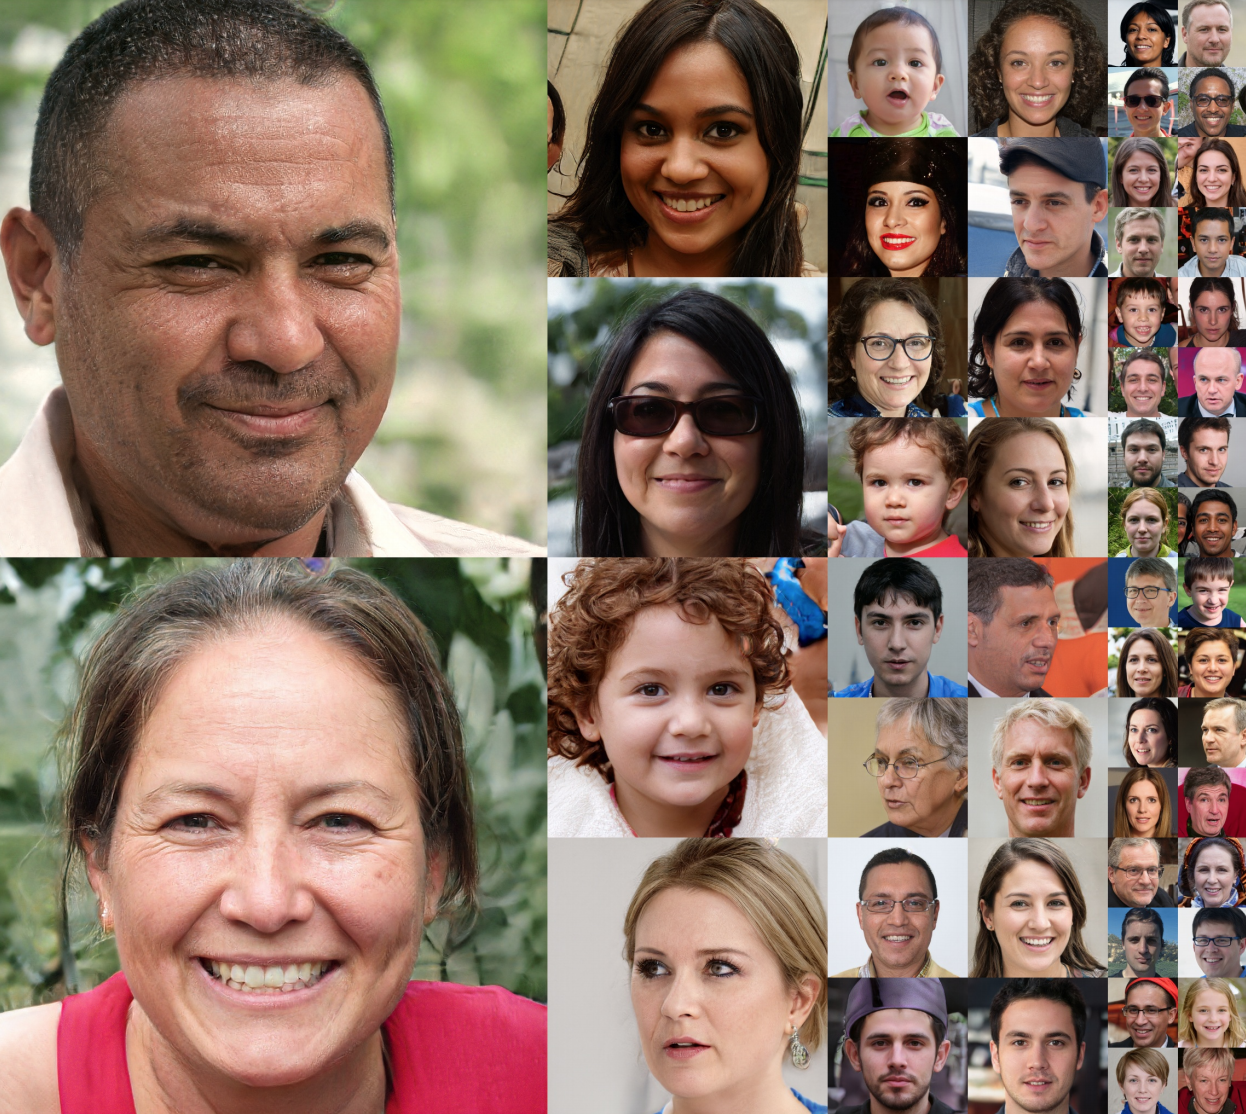
\includegraphics[width=0.5\linewidth]{ganhumans} 

    \end{figure}
\end{frame}

%%%%%%%%%%%%%%%%%%%%%%                                          About GAN Applications                   
\begin{frame}[fragile]{GAN : Applications}

    \begin{itemize}
        \item Image to image translation (in unsupervised way)
        \item blue prints to real image
        \item photo to cartoon (Facebook AI research)
        \item photo of day to night (NVIDIA Research)
        \item Creating stimulated training set (eg : face recognition problem)
        \item for imitaion learning
    \end{itemize}
\end{frame}

%%%%%%%%%%%%%%%%%%%%%%                                          About GAN Overview                   
\begin{frame}[fragile]{GAN : Overview}
 GANs has two parts: \\
    \begin{itemize}
        \item The generator : learns to generate plausible data. The generated instances become negative training examples for the discriminator.

        \item The discriminator: learns to distinguish the generator's fake data from real data. The discriminator penalizes the generator for producing implausible results.
    \end{itemize}
\end{frame}


%%%%%%%%%%%%%%%%%%%%%%                                          About GAN Training                   
\begin{frame}[fragile]{GAN : Training}
     \begin{figure}[ht]
         \hspace*{-1cm}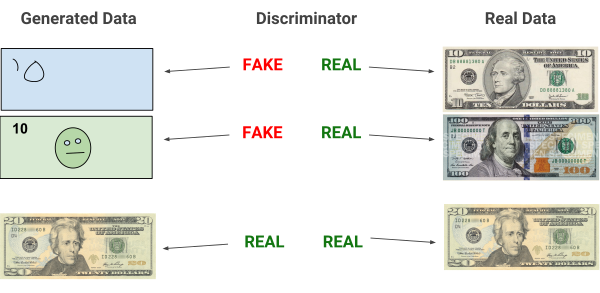
\includegraphics[width=0.8\linewidth]{gantrain} \\ \\ \\ \\ \\ 


    \end{figure}
\end{frame}

%%%%%%%%%%%%%%%%%%%%%%                                          About GAN Architecture                   
\begin{frame}[fragile]{GAN : Architecture}
     \begin{figure}[ht]
         \hspace*{-1cm}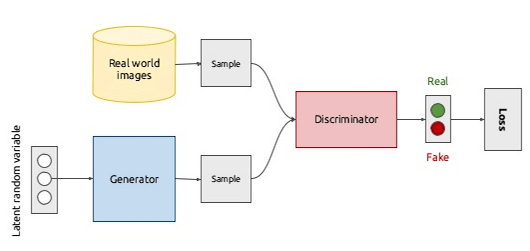
\includegraphics[width=0.8\linewidth]{ganarchitecture.png} \\ \\ \\ \\ \\ 
    \end{figure}
\end{frame}
%%%%%%%%%%%%%%%%%%%%%%%%%%%%%%%%%%%%%%%%%%%%%%%%%%%%%%%%%%%%%%%%%%%%%%